\section{Motivating Example}
\label{sec:example}

We now present some real world examples to motivate our approach. In particular, through these examples, we demonstrate that developers often ignore the tempral specifications of an API present in its documentation. We suspect the reason for this phenomena is that API documentation is often verbose and information is distributed across various
pages. For example, the PDF version of the documentation for Amazon S3 API\footnote{\url{http://awsdocs.s3.amazonaws.com/S3/latest/s3-api.pdf}} spans 278 pages. Developers do not have time and patience to go through all the documentation and miss various temporal specifications of the API, resulting in defective applications that invoke API methods in sequences prohibited by documentation. 
If we have the formal temporal specifications such kinds of defects can be detected by formal verification tools.

\begin{figure}[t]
\begin{center}
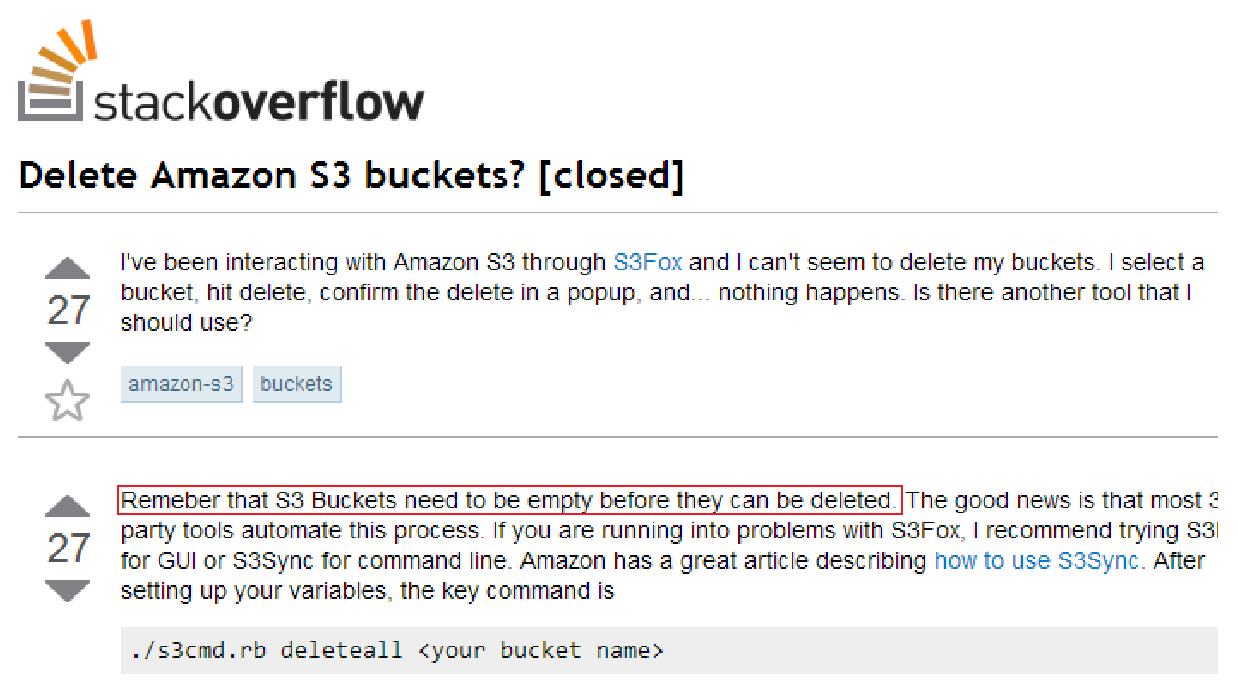
\includegraphics[scale=0.45]{Stackoverflow.eps}
\end{center}
\caption{\label{fig:Stackoverflow} The Query posted on Stackoverflow form regrading Amazon S3 REST API}
\end{figure}

Consider the question asked in \textit{Stack Overflow}~\footnote{\url{http://stackoverflow.com/}} as shown in Figure~\ref{fig:Stackoverflow}.
Stack Overflow is a question and answer site for professional and enthusiast programmers.
The query is about the delete functionality of a third-party software \CodeIn{S3Fox} to interact with \amazonAPI.
The inquisitor complains about an issue in delete bucket functionality of the \CodeIn{S3Fox}.
In particular, the issue was because the \CodeIn{S3Fox} developers overlooked the specifications in \amazon.
The document clearly states that before deleting the bucket, the objects in the buckets must be deleted. \textit{``All objects (including all objects versions and Delete Markers) in the bucket must be deleted before the bucket itself can be deleted''}.
Although the issue was fixed but notice that one of the responses on the \textit{Stack Overflow} encouraged the person asking query to switch to another product, thus potentially resulting in a loss of revenue attributed to customer dissatisfaction.
In yet another example a developer points out the financial losses he suffered because he was incorrectly using the previously described delete bucket functionality as shown in Figure~\ref{fig:example2}, \textit{(``...paying for excess stuff you don't need is simply idiotic...'')}. 


%\begin{figure}[t]
%\begin{center}
%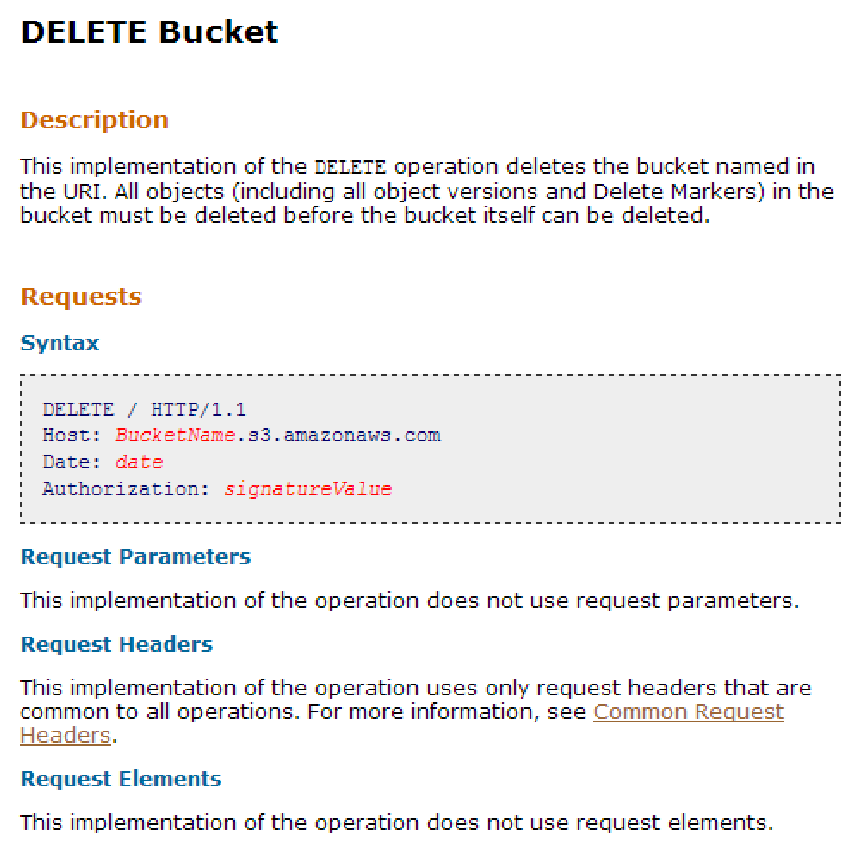
\includegraphics[scale=0.5]{AmzonS3DeleteBucketAPI.eps}
%\end{center}
%\caption{\label{fig:AmzonS3DeleteBucketAPI} The online API document for \CodeIn{DELETE Bucket} operation in Amazon S3 REST API}
%\end{figure}

Formal verification tools can be used to easily find such kind of defects.
However, formal analysis tools are not designed to work on specifications in natural languages (such as API Documents) and require the specifications in a more formal or machine understandable format. 
Thus, there is need for an approach to automatically translate the constraints described in natural language into a more formal notation. In next section, we briefly discuss the related work in this area.


\begin{figure}[t]
\begin{center}
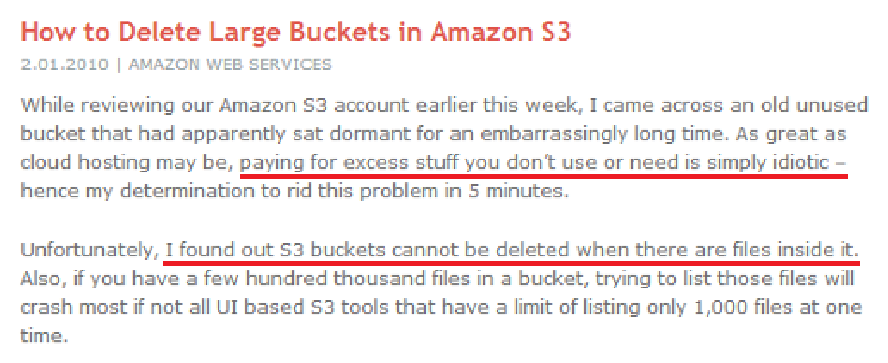
\includegraphics[scale=0.6]{Example2.eps}
\end{center}
\caption{\label{fig:example2} The experience article posted by a developer regarding Amazon S3 REST API}
\end{figure}


 








